\documentclass[tikz,border=10pt]{standalone}

\begin{document}
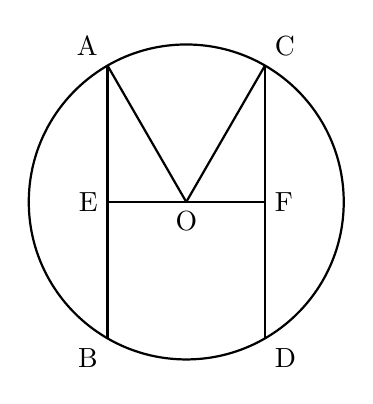
\begin{tikzpicture}[scale=1]

% 1. Draw the circle with center O (Radius = 2)
\draw[thick] (0,0) circle (2);

% 2. Define coordinates
\coordinate (O) at (0,0);
\coordinate (E) at (-1,0);
\coordinate (F) at (1,0);

% Calculating y = sqrt(2^2 - 1^2) = 1.732 for perfect connection
\coordinate (A) at (-1, 1.732);
\coordinate (B) at (-1, -1.732);
\coordinate (C) at (1, 1.732);
\coordinate (D) at (1, -1.732);

% 3. Draw the vertical chords AB and CD
\draw[thick] (A) -- (B);
\draw[thick] (C) -- (D);

% 4. Draw the horizontal segment EF through center O
\draw[thick] (E) -- (F);

% 5. Draw the segments AO and CO to complete the 'M' shape
\draw[thick] (A) -- (O);
\draw[thick] (C) -- (O);

% 6. Place labels exactly as shown in the image
\node[below] at (O) {O};
\node[above left] at (A) {A};
\node[below left] at (B) {B};
\node[above right] at (C) {C};
\node[below right] at (D) {D};
\node[left] at (E) {E};
\node[right] at (F) {F};

\end{tikzpicture}
\end{document}
